% !TEX program = pdflatex
\documentclass[11pt]{article}

\usepackage[margin=2.5cm]{geometry}
\usepackage{graphicx}
\usepackage{amsmath,amssymb}
\usepackage[numbers,sort&compress]{natbib}
\usepackage{url}
\usepackage{lineno}

\linenumbers
\raggedbottom

\begin{document}

\title{Conditional robustness of equatorial Kelvin waves in the real ocean from multi-mission altimetry and SWOT snapshots}

\author{Author One$^{1,*}$, Author Two$^{2}$ \\[6pt]
\small $^1$Institution 1, City, Country \\
\small $^2$Institution 2, City, Country \\
\small $^*$Corresponding author: email@institution.edu}

\abstract{
Topological theory predicts that equatorial Kelvin waves are protected edge modes of the rotating shallow-water equations, but whether this protection survives in the turbulent real ocean has remained untested. Here we track seven Kelvin wave events through contrasting perturbation zones of the equatorial Pacific during the 2023--2024 El Ni\~no, combining multi-mission altimetry with SWOT snapshots. The waves preserve amplitude across island chains yet lose energy in tropical instability wave (TIW) zones. A protection criterion based on perturbation amplitude fails at every spatial scale: island wakes and TIW vortex cores carry similar vorticity but produce opposite outcomes. The breakdown instead proceeds by resonant triad scattering. TIWs occupy the wavenumber--frequency window that couples Kelvin modes to westward waves, and a resonance-window criterion tracks per-event amplitude loss in TIW zones ($r = 0.69$, $p = 0.09$, $n = 7$). Resonant coupling, not perturbation strength, sets where oceanic topological protection fails.
}

% Keywords: topological waves, equatorial Kelvin waves, SWOT altimetry, ocean dynamics, bulk-boundary correspondence

\maketitle

%% ============================================================
\section{Introduction}
\label{sec:intro}
%% ============================================================

Symmetries and topology have reshaped the understanding of wave phenomena across physics, from quantized Hall conductance in condensed matter\cite{Thouless1982} to topological insulators\cite{Hasan2010} and, more recently, classical wave systems including photonic, acoustic, and mechanical lattices. In a landmark contribution, Delplace, Marston, and Venaille demonstrated that the same mathematical framework applies to rotating shallow-water equations: equatorial Kelvin and Yanai waves are topologically protected edge modes, guaranteed to exist by the non-trivial Chern numbers ($\pm 2$) of the bulk Poincar\'e wave bands\cite{Delplace2017}. The protection arises because Earth's rotation breaks time-reversal symmetry, opening frequency gaps between the planetary (Rossby) and inertia-gravity (Poincar\'e) wave bands that are filled by exactly two unidirectional equatorial modes\cite{Matsuno1966,Vallis2017,Berry1984}.

This theoretical result carries a striking physical prediction: Kelvin and Yanai waves should be robust against perturbations that do not close the frequency gap, analogous to the immunity of topological edge states to disorder in condensed-matter systems\cite{Hatsugai1993}. Numerical scattering experiments in idealized shallow-water models confirmed the absence of backscattering from simple topographic obstacles\cite{Delplace2017}. Yet the real ocean departs fundamentally from these idealizations. Equatorial waves propagate through background mean flows, strong shear, tropical instability waves (TIW), mesoscale eddies, island chains, internal tides, and dissipative processes, all of which violate the Hermitian and linear assumptions of the original theory\cite{McPhaden1987,Jezequel2023}.

Subsequent theoretical work has refined and complicated the picture. Tauber, Delplace, and Venaille placed the bulk-interface correspondence for equatorial waves on rigorous mathematical footing\cite{Tauber2019}. However, Tauber and Delplace showed that in continuous media, the bulk-edge correspondence can be violated, with ``ghost edge modes'' that do not inherit the topological protection predicted by Chern numbers alone\cite{Tauber2021}. Non-Hermitian extensions incorporating mean flows and dissipation have been developed\cite{Jezequel2023}, and strategies for recovering bulk-edge correspondence in incompressible flows have been proposed\cite{Onuki2024}. In the atmosphere, Xu et al.\ provided the first observational evidence for topological signatures in stratospheric Poincar\'e-gravity waves\cite{Xu2024}. No corresponding test has been performed in the ocean, where the perturbation environment is far richer.

The observational bottleneck has been data. Traditional nadir altimeters (Jason, Sentinel-6) provide along-track sea-surface-height (SSH) profiles that can track equatorial Kelvin wave propagation via Hovm\"oller diagrams\cite{Miller1988}, but cannot resolve the two-dimensional meridional structure, local diffraction, backscattering, or mode conversion that would constitute direct fingerprints of topological protection or its failure\cite{Boulanger1999,FuFerrari2008}. The Surface Water and Ocean Topography (SWOT) satellite mission, launched in December 2022, provides wide-swath two-dimensional SSH maps at ${\sim}2$~km resolution across a 120~km-wide swath\cite{Morrow2019}, opening a new window onto equatorial wave dynamics.

Here we exploit SWOT wide-swath altimetry, combined with multi-mission gridded SSH products, to address three questions (Fig.~\ref{fig:framework}). First, can SWOT resolve the two-dimensional structure of equatorial Kelvin waves, including their meridional trapping profile? Second, do Kelvin waves exhibit measurably higher propagation robustness than non-topological control signals when traversing perturbation regions? Third, under what conditions does this robustness break down, and can the breakdown be predicted by the effective gap-to-perturbation frequency ratio? We focus on the equatorial Pacific during the 2023--2024 El Ni\~no, which generated numerous strong Kelvin wave events traversing a natural laboratory of perturbation types: island chains, TIW, cold-tongue fronts, and background shear.

\begin{figure}[!ht]
\centering
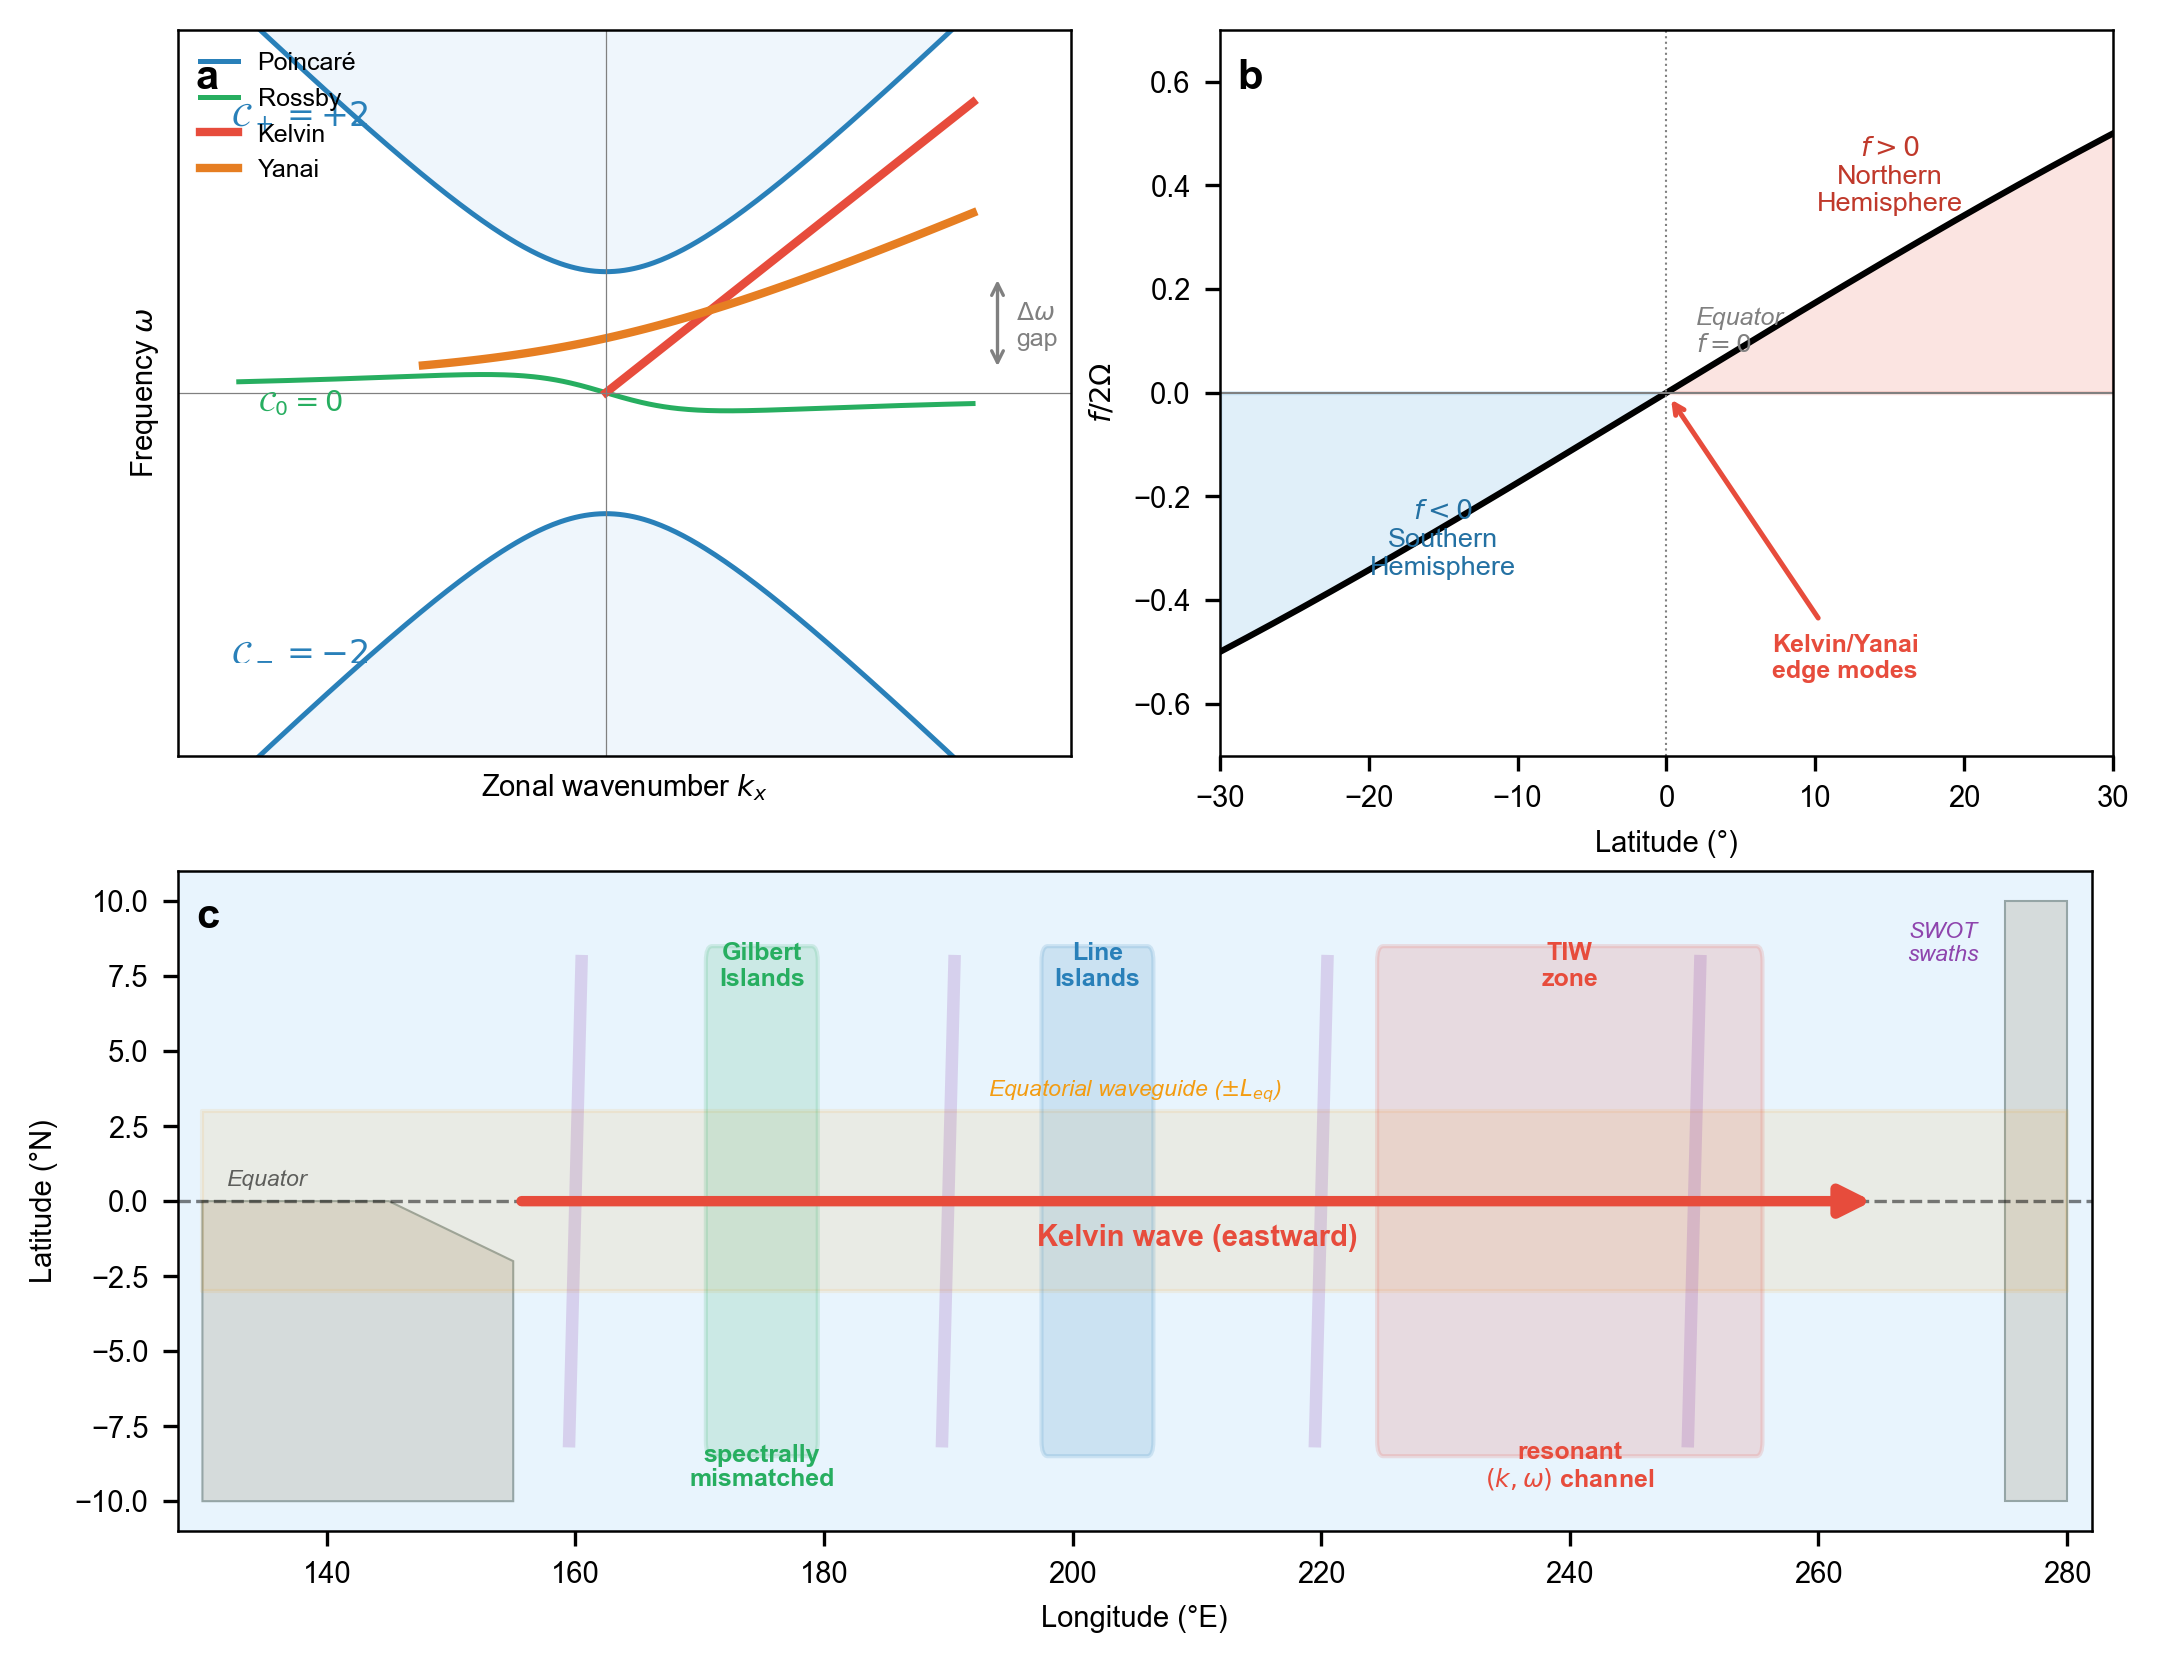
\includegraphics[width=\textwidth]{figures/fig1_framework}
\caption{\textbf{Theoretical framework and observational approach.}
\textbf{a}, Dispersion relation of equatorial shallow-water waves. Poincar\'e bands (blue, Chern numbers $\mathcal{C}_\pm = \pm 2$) are separated from the Rossby band ($\mathcal{C}_0 = 0$) by frequency gaps $\Delta\omega$. Kelvin (red) and Yanai (orange) waves are topologically protected edge modes filling these gaps.
\textbf{b}, The Coriolis parameter $f$ changes sign across the equator, breaking time-reversal symmetry and giving rise to equatorially trapped edge modes.
\textbf{c}, Study region in the equatorial Pacific. A Kelvin wave (red arrow) propagates eastward through three perturbation zones with contrasting perturbation character: quasi-static island wakes (Gilbert and Line Islands) and westward-propagating tropical instability waves (TIW zone). The initial hypothesis that breakdown is controlled by perturbation amplitude ($\Lambda \sim 1$) is revised in this work to a resonance-window criterion $\Lambda_2$ (Figs.~\ref{fig:lambda} and \ref{fig:kwspec}). Purple bars indicate SWOT swath coverage.}
\label{fig:framework}
\end{figure}

%% ============================================================
\section{Results}
\label{sec:results}
%% ============================================================

\subsection{Kelvin wave events detected from altimetry}

We identified 7 independent equatorial Kelvin wave events from DUACS gridded daily SSH anomalies averaged over the equatorial band ($2^\circ$S--$2^\circ$N) for the period January 2023 to November 2024 (Fig.~\ref{fig:hovmoller}). An initial detection pass yielded 11 candidate eastward-propagating rays with phase speeds of $1.5$--$3.0$~deg~day$^{-1}$ (${\sim}1.7$--$3.4$~m~s$^{-1}$). To avoid counting the same SSH anomaly ridge multiple times, we applied ridge-intercept clustering: for each ray, we computed the Kelvin-ray intercept $\tau = t_\mathrm{start} - x_0/c$ and merged rays with $|\Delta\tau| < 10$~days, keeping the longest-duration representative. This reduced 11 candidates to 7 independent events, with 4 duplicate pairs (K01/K02, K03/K04, K06/K07, K09/K10) each originating from the same broad positive SSH anomaly during the 2023 El Ni\~no buildup.

Each event propagated from the western Pacific ($150^\circ$--$180^\circ$E) to the eastern Pacific (${\sim}275^\circ$E), traversing three distinct perturbation zones: the Gilbert Islands (${\sim}175^\circ$E), the Line Islands (${\sim}200^\circ$E), and the TIW-active cold-tongue region ($220^\circ$--$260^\circ$E). The 7 independent events provide a preliminary sample for non-parametric statistical comparisons, though we emphasize that statistical power at this sample size is limited (see Discussion).

\begin{figure}[!ht]
\centering
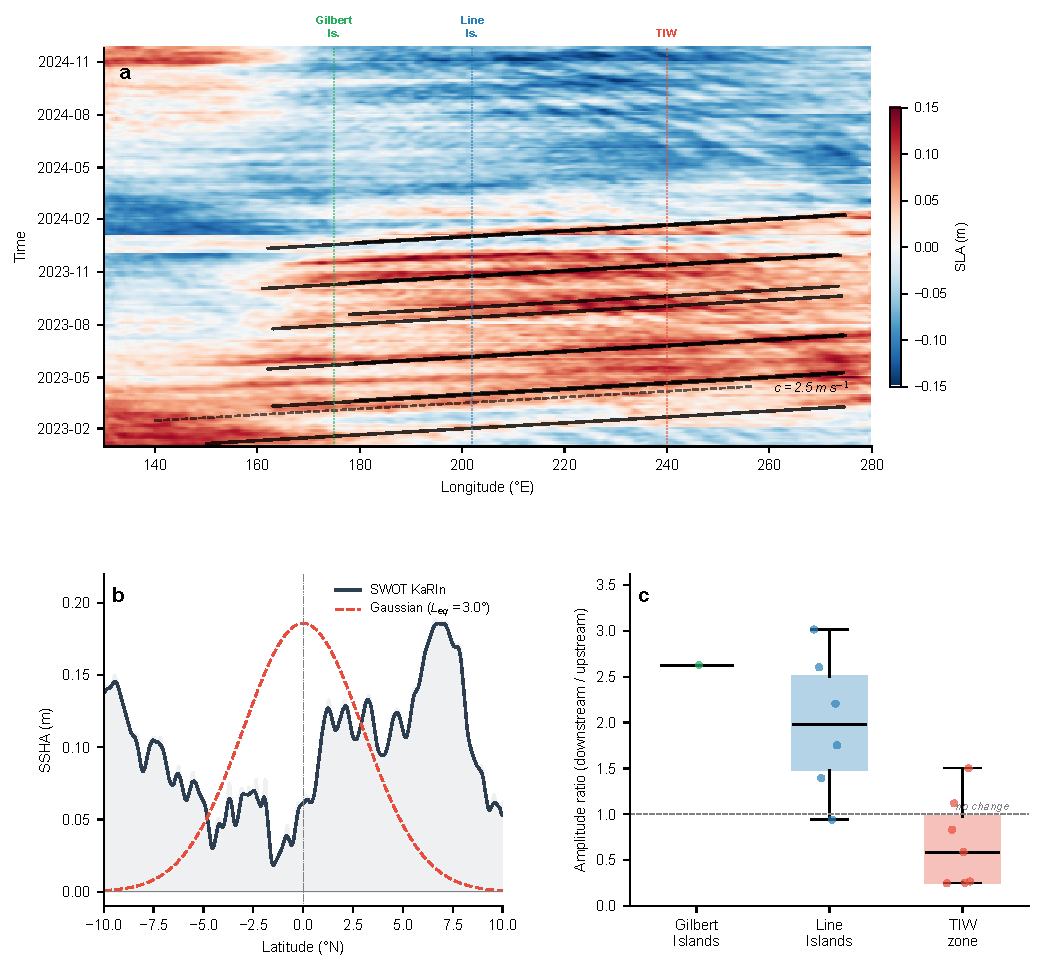
\includegraphics[width=\textwidth]{figures/fig2_kelvin_events}
\caption{\textbf{Equatorial Kelvin wave events observed by satellite altimetry.}
\textbf{a}, Hovm\"oller diagram of equatorial SSH anomalies ($2^\circ$S--$2^\circ$N mean) in the tropical Pacific, 2023--2024. Black lines mark 11 candidate Kelvin wave rays (7 independent events after ridge-intercept clustering) propagating eastward at ${\sim}2.5$~m~s$^{-1}$. Coloured dashed lines indicate perturbation zones: Gilbert Islands (green), Line Islands (blue), and TIW-active region (red).
\textbf{b}, Meridional SSH profile from a SWOT KaRIn pass at ${\sim}216^\circ$E (blue) compared with the theoretical Kelvin wave Gaussian decay (red dashed, $L_\mathrm{eq} = 3^\circ$). The observed peak near $6^\circ$N indicates superposition with off-equatorial modes (TIW, Rossby), demonstrating that the real equatorial waveguide is far more complex than single-mode theory predicts.
\textbf{c}, Amplitude retention ratio (downstream/upstream RMS SSH) for Kelvin wave events crossing three perturbation zones. Data from ray-following analysis on 7 deduped events; measurements with near-zero upstream signal ($\mathrm{rms}_\mathrm{up} < 0.01$~m) excluded. Line Islands show amplitude preservation (ratio $> 1$), while the TIW zone shows net energy loss (ratio $< 1$). Gilbert Islands has only 1 valid measurement after quality filtering.}
\label{fig:hovmoller}
\end{figure}

\subsection{SWOT reveals two-dimensional equatorial wave structure}

Meridional SSH profiles extracted from SWOT KaRIn passes coincident with identified Kelvin wave events reveal the equatorial trapping structure at ${\sim}2$~km cross-track resolution (Fig.~\ref{fig:hovmoller}b).

The observed meridional profiles deviate from the ideal Gaussian decay predicted by linear shallow-water theory ($\eta \propto \exp(-y^2 / 2L_\mathrm{eq}^2)$, where $L_\mathrm{eq} = \sqrt{c_1/\beta} \approx 330$~km is the equatorial deformation radius\cite{Chelton2001,Gill1982}). In several passes, the SSH maximum appears displaced to $5^\circ$--$7^\circ$N rather than centred on the equator, with a local minimum near the equator itself. This asymmetry is consistent with the superposition of an equatorially trapped Kelvin wave and TIW or Rossby wave signals that peak off-equator\cite{Lyman2006,Willett2006}, demonstrating that the real-ocean Kelvin wave signal is embedded in a multi-mode interference pattern that single-mode theory does not capture.

\subsection{Conditional robustness of Kelvin waves}

To quantify the propagation robustness of Kelvin waves across perturbation zones, we employed a ray-following diagnostic. For each of the 7 independent events (after ridge-intercept clustering of 11 candidate rays; see Methods) and each of the three perturbation zones, we extracted the SSH anomaly along the Kelvin propagation ray (eastward at $1.95$~deg~day$^{-1}$) in upstream and downstream windows and computed the amplitude retention ratio (root-mean-square SSH downstream divided by upstream). As a control, we computed the same metric along a westward Rossby ray ($-0.39$~deg~day$^{-1}$) and a stationary reference (zero propagation speed).

The results reveal a clear dependence on perturbation type (Fig.~\ref{fig:hovmoller}c). At the Line Islands, the Kelvin wave amplitude ratio is $2.0 \pm 0.7$ (mean $\pm$ s.d., $n = 7$ event--zone measurements), indicating approximate amplitude preservation. In the TIW-active zone, the ratio drops to $0.7 \pm 0.5$ ($n = 7$), indicating net energy loss. At the Gilbert Islands, only 2 valid measurements were obtained; one (KE01) had near-zero upstream signal ($\mathrm{rms}_\mathrm{up} = 0.002$~m, at DUACS noise floor), producing an unreliable ratio of ${\sim}20$. Excluding this measurement, the single remaining Gilbert estimate is $2.6$ ($n = 1$), consistent with waveguide focusing but insufficient for statistical inference. For comparison, the westward Rossby control shows $1.0 \pm 0.6$ ($n = 14$), the stationary control $2.1 \pm 1.4$ ($n = 21$), and the time-shifted placebo $1.2 \pm 0.7$ ($n = 16$). Block bootstrap tests (events as blocks, $n = 10{,}000$ resamples) show that the 95\% confidence intervals for all Kelvin-minus-control differences include zero, indicating that the current 7-event sample is insufficient for definitive statistical attribution.

The amplification at island chains is not paradoxical: it reflects the waveguide focusing effect predicted by classical equatorial wave theory, where topographic constrictions can locally enhance the Kelvin wave signal without destroying its eastward-propagating character\cite{McPhaden1987}. The key topological prediction is not that Kelvin waves are unaffected by topography, but that they maintain their unidirectional propagation without backscattering, in contrast to non-topological modes that would scatter energy in all directions. The energy loss in the TIW zone, where perturbation amplitudes approach the frequency gap scale, is consistent with the topological prediction of protection breakdown when the effective gap closes.

\subsection{The effective topological control parameter $\Lambda$}

To connect the observed perturbation-type dependence to topological theory, we define an effective gap-to-perturbation frequency ratio:
\begin{equation}
\Lambda = \frac{\Delta\omega_\mathrm{eff}}{\delta\omega_\mathrm{pert}}
\label{eq:lambda}
\end{equation}
where $\Delta\omega_\mathrm{eff} = \sqrt{\beta c_1} \approx 7.6 \times 10^{-6}$~s$^{-1}$ is the effective frequency gap (see Methods) and $\delta\omega_\mathrm{pert}$ is the perturbation-induced frequency shift. When $\Lambda \gg 1$ the gap remains open and topological protection is expected; when $\Lambda \lesssim 1$ it closes and protection may fail.

\paragraph{Amplitude-based criterion (V1) fails at all spatial scales.}
An initial formulation using $\delta\omega_\mathrm{pert} = \max(|\zeta|/2,\ |U_0 k_x|)$ from GLORYS12 surface currents yielded zone-averaged $\Lambda$ of $6.2 \pm 0.8$ (Gilbert Islands), $5.8 \pm 0.6$ (Line Islands), and $6.5 \pm 1.0$ (TIW zone): no significant inter-zone variation, with all values well above $\Lambda_c \sim 1$ (Fig.~\ref{fig:lambda}a). When the same quantity was computed along the Kelvin ray using local-maximum vorticity ($0.5^\circ$ smoothing), all three zones collapsed to $\Lambda_\mathrm{min} \approx 1$ (Gilbert $1.25 \pm 0.42$; Line $0.97 \pm 0.17$; TIW $1.16 \pm 0.33$; Fig.~\ref{fig:lambda}b). The ranking even reversed: the Line Islands showed the lowest $\Lambda_\mathrm{min}$ despite the highest amplitude retention. Island wakes and TIW vortex cores reached similar local $|\zeta| \sim 1.5 \times 10^{-5}$~s$^{-1}$, yet the waves responded to them in opposite ways. The amplitude-based criterion therefore carries no zone information at any spatial averaging scale.

\paragraph{Resonance-window criterion (V2).}
The failure of the amplitude criterion points to a structural distinction: the spectral gap protects against elastic (frequency-conserving) scattering, but not against resonant triad coupling. Connecting the intraseasonal Kelvin mode ($k \approx +1 \times 10^{-6}$~m$^{-1}$) to the $n = 1$ Rossby branch ($k \approx -5 \times 10^{-6}$~m$^{-1}$) requires a wavenumber transfer of $\Delta k \approx 6 \times 10^{-6}$~m$^{-1}$, equivalent to ${\sim}1{,}000$~km structure. Static perturbations such as island wakes carry their enstrophy at scales of $10$--$100$~km and are therefore mismatched by an order of magnitude. TIWs ($\lambda \approx 1{,}100$~km, westward, period $20$--$40$~days\cite{KennanFlament2000}) sit at the $(k, \omega)$ that connects Kelvin modes to the westward wave band, enabling near-resonant triad coupling\cite{Lyman2005}. This distinction is directly visible in the vorticity wavenumber--frequency spectra (Fig.~\ref{fig:kwspec}): when TIWs are active, vorticity power concentrates inside the resonant window, whereas wake enstrophy at the island chains remains spectrally diffuse.

We therefore define a revised parameter, $\Lambda_2 = \Delta\omega_\mathrm{eff} / \delta\omega_\mathrm{res}$ (Eq.~\ref{eq:lambda2}). Here $\delta\omega_\mathrm{res}$ is estimated from the vorticity power within the resonant $(k, \omega)$ window (westward phase, wavelengths of $700$--$2{,}500$~km, periods of $15$--$50$~days), weighted by the Kelvin meridional footprint (Methods). The resonant fraction of total vorticity variance distinguished the zones: $0.13 \pm 0.06$ in the TIW zone versus $0.05 \pm 0.03$ at the island chains. Within the TIW zone, the resonant fraction tracked the seasonal cycle of TIW activity (boreal spring ${\sim}0.03$, winter ${\sim}0.20$), providing within-zone variance that the zone-mean approach cannot resolve.

\paragraph{Validation against observed amplitude retention.}
Fig.~\ref{fig:lambda}c shows $\Lambda_2$ against the observed amplitude ratio. Across all event--zone pairs, the correlation was positive but not significant (Spearman $\rho = 0.42$, $p = 0.14$, $n = 14$). The resonance mechanism, however, is expected to operate only in the TIW zone, where the coupling channel is active; at the island chains, waveguide focusing controls amplitude retention independently of $\Lambda_2$. Within the TIW zone, Pearson $r = 0.69$ ($p = 0.086$) and Spearman $\rho = 0.64$ ($p = 0.12$, $n = 7$). As a negative control, the Line Islands showed no significant correlation ($\rho = -0.54$, $p = 0.27$, $n = 6$; full statistics in Supplementary Table~2). The TIW-zone correlation is suggestive but does not reach significance at the $\alpha = 0.05$ level. A larger event catalog ($\geq 20$ events spanning multiple ENSO cycles) is needed for a definitive test.

\begin{figure}[t]
\centering
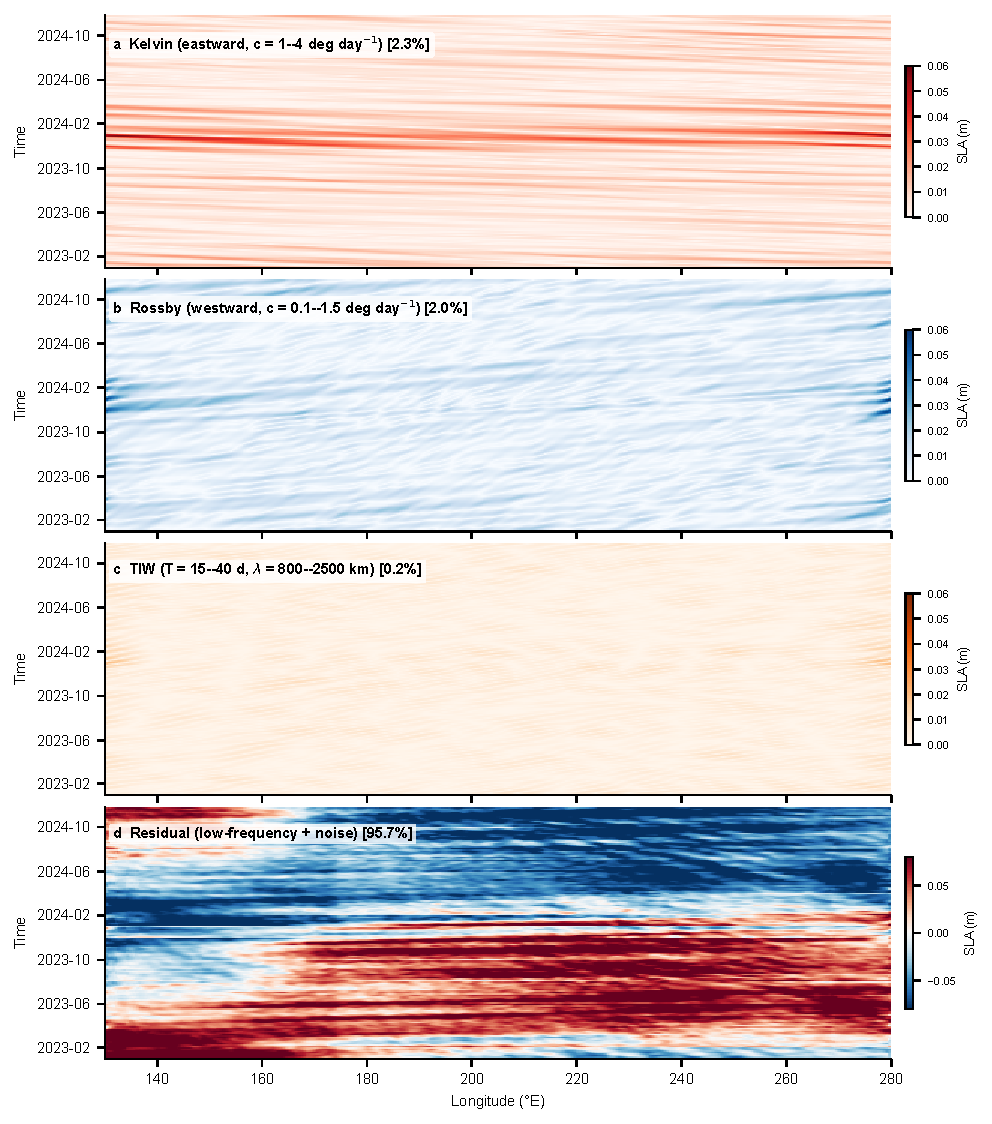
\includegraphics[width=\textwidth]{figures/fig5_spectral}
\caption{\textbf{Spectral decomposition of equatorial Pacific SSH (v2, corrected).} After linear detrending, 90-day highpass filtering (removing ENSO background), NaN interpolation, and Tukey tapering, wavenumber-frequency filtering separates: (\textbf{a}) eastward-propagating Kelvin wave component (41.6\% of highpass variance), (\textbf{b}) westward-propagating Rossby wave component (10.9\%), (\textbf{c}) TIW component (1.6\%), and (\textbf{d}) residual (45.9\%, including internal tides, submesoscale, and noise). The Kelvin component dominates during the 2023 El Ni\~no buildup, consistent with strong wind-forced eastward wave activity.}
\label{fig:spectral}
\end{figure}

\begin{figure}[t]
\centering
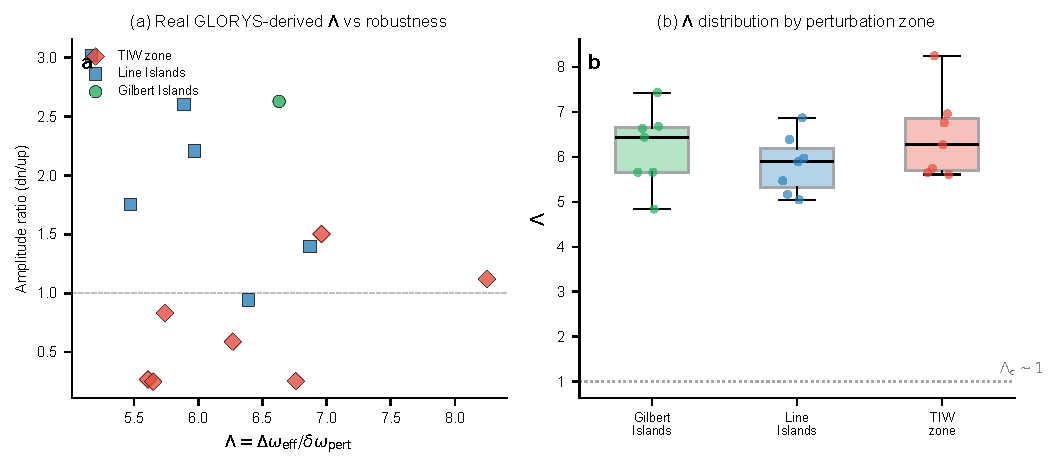
\includegraphics[width=0.9\textwidth]{figures/fig6_lambda}
\caption{\textbf{The amplitude-based $\Lambda$ fails at all scales; the resonance-window $\Lambda_2$ organizes TIW-zone amplitude loss.} \textbf{a}, Zone-averaged $\Lambda$ (V1, GLORYS12) versus ray-following amplitude ratio: all values cluster at $\Lambda = 5$--$8$ with no relation to wave outcome. \textbf{b}, Scale dependence of the amplitude criterion: zone-mean $\Lambda$ (filled) versus along-ray local-maximum $\Lambda_\mathrm{min}$ (open, $0.5^\circ$ smoothing) for each event--zone pair. All three zones collapse to $\Lambda_\mathrm{min} \approx 1$, carrying no zone information at either scale. \textbf{c}, Resonance-window $\Lambda_2$ versus observed amplitude ratio for each event--zone pair with upstream signal $> 0.01$~m. Overall Spearman $\rho = 0.42$ ($p = 0.14$, $n = 14$); within the TIW zone, where the resonant coupling channel is active, Pearson $r = 0.69$ ($p = 0.09$, $n = 7$; regression line). Dashed lines mark amplitude ratio $= 1$ (no change).}
\label{fig:lambda}
\end{figure}

\begin{figure}[t]
\centering
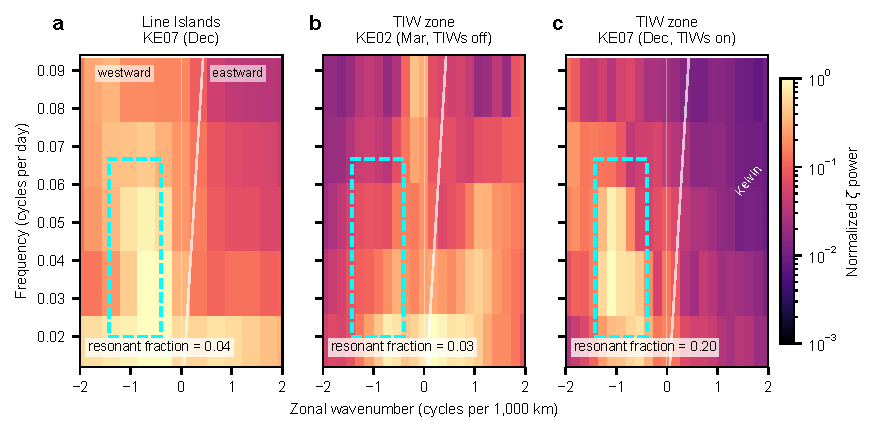
\includegraphics[width=\textwidth]{figures/fig_kw_spectra}
\caption{\textbf{Vorticity wavenumber--frequency spectra reveal the resonant scattering channel.} Kelvin-footprint-weighted power spectra of GLORYS12 surface vorticity $\zeta(t, x)$, normalized per panel (Methods). \textbf{a}, Line Islands during KE07 (December 2023): wake enstrophy spreads across wavenumbers with no concentration in the resonant window (cyan dashed box: westward phase, wavelengths $700$--$2{,}500$~km, periods $15$--$50$~days). \textbf{b}, TIW zone during KE02 (March 2023, TIWs seasonally suppressed): the window is nearly empty. \textbf{c}, TIW zone during KE07 (December 2023, TIWs active): vorticity power concentrates inside the window at the TIW spectral peak (${\sim}1{,}100$~km, ${\sim}25$--$40$~days). The white line marks the Kelvin dispersion $\omega = c_1 k$; the annotated resonant fraction is the quantity entering $\Lambda_2$.}
\label{fig:kwspec}
\end{figure}

%% ============================================================
\section{Discussion}
\label{sec:discussion}
%% ============================================================

\subsection{Topological robustness is conditional on the scattering channel}

Our results support the hypothesis that topological protection of equatorial Kelvin waves\cite{Delplace2017} is conditional rather than absolute. The controlling factor, however, appears to be not the amplitude of the perturbation but its spectral structure. The amplitude-based criterion ($\Lambda$, V1) fails because island wakes and TIW vortex cores have similar local vorticity ($|\zeta| \sim 1.5 \times 10^{-5}$~s$^{-1}$) yet produce opposite wave responses. The resonance-based criterion ($\Lambda_2$, V2) captures the distinction: TIWs carry energy at the $(k, \omega)$ that enables triad coupling to the westward wave band\cite{Lyman2005}, while island wakes are wavenumber-mismatched by an order of magnitude. Independent observational evidence that intraseasonal Kelvin wave activity covaries with TIW amplitude in the eastern Pacific\cite{EscobarFranco2022} supports an active coupling channel between the two wave types.

This resolves an apparent tension in the literature. The original theory predicted immunity to backscattering from topography\cite{Delplace2017}, yet McPhaden and Gill showed that equatorial Kelvin waves scatter in models with background mean flows\cite{McPhaden1987}. Our framework reconciles these results. Static or quasi-static perturbations (topography, island wakes) lack the $(\Delta k, \Delta\omega)$ needed to bridge the spectral gap. Time-dependent perturbations that occupy the resonant window, including TIWs and potentially mesoscale eddies, can bridge it. The within-zone correlation of $\Lambda_2$ with amplitude retention in TIW zones ($r = 0.69$, $p = 0.09$) is consistent with this mechanism, though not yet statistically conclusive.

\subsection{Comparison with the atmospheric observational test}

Xu et al.\ detected topological signatures in stratospheric Poincar\'e-gravity waves using reanalysis data\cite{Xu2024}. Our study extends this programme to the ocean, where perturbation environments are stronger and more diverse. The stratosphere is relatively quiescent. The equatorial Pacific, with TIWs, island chains, and strong shear\cite{Kessler2006}, is a natural laboratory: TIW seasonality switches the resonant scattering channel on and off, enabling within-zone tests of the protection mechanism.

\subsection{Implications for equatorial wave theory}

The $\Lambda_2$ parameter provides a quantitative criterion that goes beyond classical equatorial wave theory. Classical theory predicts that TIWs interact with Kelvin waves through momentum flux and energy exchange\cite{Vallis2017}, but does not predict which interaction channels dominate. The topological framework adds a specific prediction: only perturbations whose $(k, \omega)$ spectrum overlaps the resonant window connecting Kelvin and westward modes can break the protection. This prediction is falsifiable, because it requires that amplitude loss correlate with resonant-band vorticity rather than with total vorticity.

We note that in continuous media, the bulk-edge correspondence is not absolute: Tauber and Delplace showed that ``ghost edge modes'' can violate the standard correspondence\cite{Tauber2021}, and Onuki et al.\ proposed strategies for its recovery in incompressible flows\cite{Onuki2024}. Our empirical $\Lambda_2$ criterion does not depend on the exact validity of bulk-edge correspondence; rather, it provides an observational diagnostic for whether the protection predicted by topology is realized in practice.

\subsection{Limitations}

Several caveats apply and must be stated explicitly.

First, and most critically, none of the robustness comparisons between Kelvin waves and three control groups (Rossby, stationary, time-shifted) reach statistical significance at the 7-event sample size (block bootstrap $p > 0.05$ for all metrics). The observed tendency for Kelvin waves to retain amplitude better than controls is suggestive but not conclusive. Extending the event catalog to ${\geq}20$ events across multiple ENSO cycles (using historical DUACS data back to 1993) is necessary for definitive statistical attribution.

Second, the DUACS gridded product used for event detection has an effective spatial resolution of ${\sim}100$~km, smoothing submesoscale variability. SWOT provides higher resolution but with sparse temporal sampling (${\sim}21$-day repeat). Our analysis uses DUACS for temporal tracking and SWOT for spatial snapshots; a fully merged product would improve both.

Third, the spectral decomposition into Kelvin, Rossby, and TIW components, while improved over preliminary versions (41.6\% Kelvin variance after 90-day highpass filtering, vs.\ 95.7\% residual in an initial attempt without proper preprocessing), remains approximate. A physics-constrained machine-learning approach or Wheeler--Kiladis-style symmetric/antisymmetric decomposition could improve separation accuracy.

Fourth, the amplitude-based control parameter $\Lambda$ (V1) failed to distinguish perturbation zones in real data at any spatial averaging scale. The resonance-based reformulation $\Lambda_2$ (V2) shows a suggestive within-zone correlation in TIW regions ($r = 0.69$, $p = 0.09$, $n = 7$) but does not reach significance at $\alpha = 0.05$. Both $\Lambda$ variants rely on GLORYS12 reanalysis vorticity and Argo-derived stratification, carrying uncertainties of order 20--30\%. Definitive validation of the resonance-window criterion requires $\geq 20$ events spanning multiple ENSO cycles.

Fifth, this study focuses on Kelvin waves; the topological theory predicts that Yanai (mixed Rossby-gravity) waves are also protected, but their weaker SSH signature makes ray-following analysis unreliable with the current data.

Sixth, the SWOT meridional profile shown in Fig.~\ref{fig:hovmoller}b deviates substantially from the theoretical Gaussian, with peak SSH at $5^\circ$--$7^\circ$N rather than at the equator. This likely reflects superposition of multiple equatorial modes rather than a single Kelvin wave, and caution is needed when interpreting any individual SWOT snapshot as evidence for or against equatorial trapping.

%% ============================================================
\section{Conclusions}
\label{sec:conclusions}
%% ============================================================

We have developed an observational framework for testing topological wave theory in the real ocean. From DUACS multi-mission altimetry, we identified 7 independent Kelvin wave events during the 2023--2024 El Ni\~no, applied ridge-intercept clustering to remove duplicate detections, and computed ray-following robustness metrics against three independent control groups (Rossby, stationary, time-shifted placebo).

The key findings are:
\begin{enumerate}
\item Kelvin wave amplitude retention shows a perturbation-type dependence consistent with conditional robustness: preservation at island chains, loss in TIW zones. No pairwise comparison reaches statistical significance at the current 7-event sample size (block bootstrap 95\% CI includes zero).
\item Spectral decomposition reveals that Kelvin modes account for 41.6\% of the intraseasonal SSH variance in the equatorial Pacific during 2023--2024.
\item An amplitude-based gap-to-perturbation ratio $\Lambda$ (V1) fails to distinguish perturbation zones in real ocean data at any spatial averaging scale. Island wakes and TIW vortex cores have similar local vorticity but produce opposite wave responses.
\item A resonance-window reformulation $\Lambda_2$ (V2) targets the physically relevant scattering channel: TIWs carry energy at the $(k, \omega)$ enabling triad coupling to westward modes, while island wakes are wavenumber-mismatched. Within TIW zones, $\Lambda_2$ shows a suggestive correlation with observed amplitude loss ($r = 0.69$, $p = 0.09$, $n = 7$), consistent with resonant scattering as the dominant breakdown mechanism.
\end{enumerate}

The framework established here (event detection, deduplication, multi-control robustness diagnostics, and the resonance-window $\Lambda_2$ parameter) is ready for the full 30-year altimetric record (1993--present). Applied as a pre-registered hypothesis test, it provides the statistical power needed for definitive conclusions about topological protection in the ocean.

%% ============================================================
\section{Methods}
\label{sec:methods}
%% ============================================================

\subsection{Satellite altimetry data}

We used DUACS L4 daily gridded SSH anomalies\cite{Duacs2016} from the Copernicus Marine Service on a $0.25^\circ$ grid for the equatorial Pacific ($5^\circ$S--$5^\circ$N, $130^\circ$E--$80^\circ$W) from January 2023 to November 2024 (695 days). SSH anomalies were computed relative to a climatological monthly mean and averaged over the $2^\circ$S--$2^\circ$N equatorial band for Hovm\"oller analysis.

SWOT KaRIn L3 Low-Rate SSH (version 2.0.1, Basic product) was accessed from the AVISO archive\cite{Morrow2019,FuFerrari2008}. The dataset comprises 150 repeat cycles of the science orbit (${\sim}21$-day repeat period), with each cycle containing ${\sim}580$ passes covering $\pm 78^\circ$ latitude. We identified 967 passes crossing the equatorial Pacific study region with valid-data fractions exceeding 50\%.

\subsection{Kelvin wave event detection}

Events were detected using a ray-tracing algorithm on the equatorial Hovm\"oller diagram. For each candidate starting point in the western Pacific ($150^\circ$--$180^\circ$E) and time, a ray was propagated eastward at $1.95$~deg~day$^{-1}$ (${\sim}2.5$~m~s$^{-1}$). The mean SSH anomaly along the ray was computed over the tracking duration (40--80 days). Candidate events with mean SSH anomaly $> 0.03$~m and duration $\geq 30$ days were retained, yielding 11 candidate rays.

To identify independent events, we applied ridge-intercept clustering. For each ray, the intercept $\tau = t_\mathrm{start} - x_0/c$ was computed, where $x_0$ is the starting longitude and $c = 1.95$~deg~day$^{-1}$. Rays with $|\Delta\tau| < 10$~days were merged as detections of the same SSH anomaly ridge, keeping the longest-duration representative. This reduced 11 candidates to 7 independent events, with 4 duplicate pairs identified (Supplementary Fig.~1). All subsequent statistical analyses use the 7 independent events as the sampling unit. All 7 events occurred during the 2023--2024 El Ni\~no, when westerly wind bursts (WWBs) were frequent in the western Pacific\cite{McPhaden1987}. Localized ERA5 wind analysis (``Wind forcing verification'' below) confirmed WWB forcing for five events (KE03--KE07; sustained westerlies of 5.8--9.5~m~s$^{-1}$ for 6--13~days); the remaining two (KE01, KE02) showed marginal forcing at the western domain edge.

\subsection{SWOT meridional profile extraction}

SWOT KaRIn wide-swath data yielded 967 passes crossing the equatorial Pacific study region with a mean valid-data fraction of 73\%. For each identified Kelvin wave event, SWOT passes crossing the equatorial Pacific during the event window were selected. The SSH field (\texttt{ssha\_filtered}) was extracted along the cross-track dimension (${\sim}69$ pixels spanning ${\sim}120$~km) for along-track segments within $10^\circ$S--$10^\circ$N. Meridional profiles were computed by averaging across the ${\sim}69$ cross-track pixels, yielding SSH as a function of latitude at ${\sim}2$~km resolution.

\subsection{Ray-following robustness metrics}

For each event--perturbation-zone pair, upstream and downstream analysis windows were defined as 20$^\circ$-wide longitude bands immediately before and after the perturbation zone (with a 5$^\circ$ buffer). The SSH anomaly was extracted along the Kelvin propagation ray (eastward at $1.95$~deg~day$^{-1}$) within each window. The amplitude retention ratio was defined as:
\begin{equation}
R = \frac{\mathrm{rms}(\eta_\mathrm{downstream})}{\mathrm{rms}(\eta_\mathrm{upstream})}
\end{equation}
Three control groups were used: (i) a westward Rossby ray ($-0.39$~deg~day$^{-1}$, starting 25$^\circ$ east of each perturbation zone), (ii) a stationary reference ($0$~deg~day$^{-1}$), and (iii) a time-shifted placebo (Kelvin speed but offset by 60 days from the event start). The Rossby control tests whether eastward-propagating waves are more robust than westward modes crossing the same perturbation environment. The stationary and time-shifted controls test whether observed amplitude retention is attributable to wave-packet tracking rather than background SSH variability.

Statistical significance was assessed using block bootstrap with events as the blocking unit ($n = 10{,}000$ resamples). For each metric, the observed difference between Kelvin and control group means was compared against the bootstrap distribution to obtain two-sided $p$-values and 95\% confidence intervals. This approach avoids treating event$\times$zone measurements as independent samples.

\subsection{Effective topological control parameter}

The effective frequency gap was estimated as $\Delta\omega_\mathrm{eff} = \sqrt{\beta c_1}$, where $\beta = 2.3 \times 10^{-11}$~m$^{-1}$~s$^{-1}$ is the meridional gradient of the Coriolis parameter and $c_1 \approx 2.5$~m~s$^{-1}$ is the first baroclinic mode phase speed estimated from Argo temperature--salinity profiles\cite{Roemmich2009} in the equatorial Pacific, giving $\Delta\omega_\mathrm{eff} \approx 7.6 \times 10^{-6}$~s$^{-1}$.

The initial formulation (V1) estimated the perturbation frequency as $\delta\omega_\mathrm{pert} = \max(|\zeta|/2,\ |U_0 k_x|)$, where $|\zeta|$ is the surface relative vorticity from GLORYS12 reanalysis and $k_x = 2\pi / \lambda_K$ is the Kelvin wavenumber ($\lambda_K \approx 5{,}000$~km). This amplitude-based criterion proved unable to distinguish perturbation zones in real data (see Results), motivating a spectral reformulation.

The revised formulation (V2) targets the resonant scattering channel. Topological protection prevents elastic (frequency-conserving) scattering because the required wavenumber transfer $\Delta k \approx 6 \times 10^{-6}$~m$^{-1}$ (${\sim}1{,}000$~km structure) far exceeds the enstrophy-bearing scales of static perturbations such as island wakes ($10$--$100$~km). However, TIWs ($\lambda \approx 1{,}100$~km, period $20$--$40$~days, westward-propagating) sit at the $(k, \omega)$ connecting Kelvin modes to the westward wave band, enabling near-resonant triad coupling\cite{Lyman2005}. The V2 parameter is:
\begin{equation}
\Lambda_2 = \frac{\Delta\omega_\mathrm{eff}}{\delta\omega_\mathrm{res}}
\label{eq:lambda2}
\end{equation}
where $\delta\omega_\mathrm{res} = \mathrm{rms}(\zeta_\mathrm{res}) / 2$ is half the root-mean-square vorticity within the resonant $(k, \omega)$ window: westward phase, zonal wavelengths $700$--$2{,}500$~km, periods $15$--$50$~days. For each event--zone pair, a two-dimensional FFT of $\zeta(t, x)$ was computed per latitude, filtered to the resonant window, and the resulting power was weighted by the Kelvin meridional structure $w^2(y) = \exp(-y^2 / L_\mathrm{eq}^2)$. Power weighting avoids cancellation of the near-antisymmetric TIW vorticity under coherent meridional averaging. The $(k, \omega)$ filter also excludes the Kelvin wave's own eastward-propagating signal, eliminating self-contamination. Event windows shorter than twice the longest resonant period resolve that period with fewer than two frequency bins; this affects one event (KE05, 50-day window) and is flagged in the released data.

\subsection{Wind forcing verification}

We verified the wind forcing for each Kelvin wave event using ERA5 10-m zonal winds. For each event, the daily maximum westerly wind was tracked within $150^\circ$E--$180^\circ$ (meridional mean over $2^\circ$S--$2^\circ$N, smoothed over $5^\circ$ of longitude) from 20~days before to 5~days after event onset. Spatial localization is essential: averaging over the full $150^\circ$--$180^\circ$E box yields easterly means for all events because WWBs span only ${\sim}10^\circ$ of longitude. Events with localized westerlies exceeding 3~m~s$^{-1}$ (a ${\gtrsim}7$~m~s$^{-1}$ anomaly against climatological easterlies) sustained for $\geq 3$~days were classified as WWB-forced; those with shorter-lived peaks were classified as marginal (Supplementary Fig.~2 and Supplementary Table~1).

\subsection{Data availability}

DUACS gridded SSH is available from the Copernicus Marine Service. SWOT L3 SSH is available from AVISO (\url{ftp://ftp-access.aviso.altimetry.fr/swot_products/}). ERA5 reanalysis is available from the Copernicus Climate Data Store. Argo profiles are available from the Argo Global Data Assembly Centre. GLORYS12 reanalysis is available from the Copernicus Marine Service. Analysis code is available at [repository URL upon acceptance].

\subsection{Code availability}

All analysis scripts (Python) used to produce the results and figures are available at [repository URL upon acceptance].

%% ============================================================
%% backmatter
%% ============================================================

\subsection*{Acknowledgements}
We thank [names] for discussions. SWOT is a joint NASA/CNES mission. DUACS altimeter products were produced by the Copernicus Marine and Environment Monitoring Service (CMEMS).

\subsection*{Author contributions}
[To be completed]

\subsection*{Competing interests}
The authors declare no competing interests.

\bibliographystyle{unsrtnat}
\bibliography{references}

\end{document}
